% This is the Reed College LaTeX thesis template. Most of the work 
% for the document class was done by Sam Noble (SN), as well as this
% template. Later comments etc. by Ben Salzberg (BTS). Additional
% restructuring and APA support by Jess Youngberg (JY).
% Your comments and suggestions are more than welcome; please email
% them to cus@reed.edu
%
% See http://web.reed.edu/cis/help/latex.html for help. There are a 
% great bunch of help pages there, with notes on
% getting started, bibtex, etc. Go there and read it if you're not
% already familiar with LaTeX.
%
% Any line that starts with a percent symbol is a comment. 
% They won't show up in the document, and are useful for notes 
% to yourself and explaining commands. 
% Commenting also removes a line from the document; 
% very handy for troubleshooting problems. -BTS

% As far as I know, this follows the requirements laid out in 
% the 2002-2003 Senior Handbook. Ask a librarian to check the 
% document before binding. -SN

%%
%% Preamble
%%
% \documentclass{<something>} must begin each LaTeX document
\documentclass[12pt,twoside]{reedthesis}
% Packages are extensions to the basic LaTeX functions. Whatever you
% want to typeset, there is probably a package out there for it.
% Chemistry (chemtex), screenplays, you name it.
% Check out CTAN to see: http://www.ctan.org/
%%
\usepackage{graphicx,latexsym} 
\usepackage{amssymb,amsthm,amsmath}
\usepackage{longtable,booktabs,setspace} 
\usepackage{chemarr} %% Useful for one reaction arrow, useless if you're not a chem major
\usepackage{url}
\usepackage{natbib}
\usepackage[protrusion=true,expansion=true]{microtype}
\usepackage{hyperref}
\hypersetup{
    backref=true,
    bookmarks=true,         % show bookmarks bar?
    unicode=false,          % non-Latin characters in Acrobat�s bookmarks
    pdftoolbar=true,        % show Acrobat�s toolbar?
    pdfmenubar=true,        % show Acrobat�s menu?
    pdffitwindow=false,     % window fit to page when opened
    pdfstartview={FitH},    % fits the width of the page to the window
    pdftitle={My title},    % title
    pdfauthor={Author},     % author
    pdfsubject={Subject},   % subject of the document
    pdfcreator={Creator},   % creator of the document
    pdfproducer={Producer}, % producer of the document
    pdfkeywords={keyword1} {key2} {key3}, % list of keywords
    pdfnewwindow=true,      % links in new window
    colorlinks=false,       % false: boxed links; true: colored links
    linkcolor=red,          % color of internal links (change box color with linkbordercolor)
    citecolor=green,        % color of links to bibliography
    filecolor=magenta,      % color of file links
    urlcolor=cyan           % color of external links
}
\urlstyle{same}
%\usepackage[hypcap]{caption}
 %\usepackage{} % other fonts are available like times, bookman, charter, palatino

\title{An Open Science Electrophysiology Study of\\Anxiety and Commission Errors}
\author{Melissa D. Lewis}
% The month and year that you submit your FINAL draft TO THE LIBRARY (May or December)
\date{May 2013}
\division{Philosophy, Religion, Psychology, and Linguistics}
\advisor{Michael Pitts}
%If you have two advisors for some reason, you can use the following
%\altadvisor{Your Other Advisor}
%%% Remember to use the correct department!
\department{Psychology}
% if you're writing a thesis in an interdisciplinary major,
% uncomment the line below and change the text as appropriate.
% check the Senior Handbook if unsure.
%\thedivisionof{The Established Interdisciplinary Committee for}
% if you want the approval page to say "Approved for the Committee",
% uncomment the next line
%\approvedforthe{Committee}

\setlength{\parskip}{0pt}
%%
%% End Preamble
%%
%% The fun begins:
\begin{document}

  \maketitle
  \frontmatter % this stuff will be roman-numbered
  \pagestyle{empty} % this removes page numbers from the frontmatter

% Acknowledgements (Acceptable American spelling) are optional
% So are Acknowledgments (proper English spelling)
    \chapter*{Acknowledgements}
	I want to thank a few people.

% The preface is optional
% To remove it, comment it out or delete it.
    \chapter*{Preface}
	This is an example of a thesis setup to use the reed thesis document class.

    \tableofcontents
% if you want a list of tables, optional
    \listoftables
% if you want a list of figures, also optional
    \listoffigures

% The abstract is not required if you're writing a creative thesis (but aren't they all?)
% If your abstract is longer than a page, there may be a formatting issue.
    \chapter*{Abstract}
	The preface pretty much says it all.
	
	\chapter*{Dedication}
	You can have a dedication here if you wish.

  \mainmatter % here the regular arabic numbering starts
  \pagestyle{fancyplain} % turns page numbering back on

%The \introduction command is provided as a convenience.
%if you want special chapter formatting, you'll probably want to avoid using it altogether

\chapter*{Introduction}
         \addcontentsline{toc}{chapter}{Introduction}
	\chaptermark{Introduction}
	\markboth{Introduction}{Introduction}
	% The three lines above are to make sure that the headers are right, that the intro gets included in the table of contents, and that it doesn't get numbered 1 so that chapter one is 1.

% Double spacing: if you want to double space, or one and a half 
% space, uncomment one of the following lines. You can go back to 
% single spacing with the \singlespacing command.
% \singlespacing
%\doublespacing
\onehalfspace

	\section{The Neural Basis of Error Monitoring and Defensive Motivation}
	
		\subsection{Error Monitoring}
		The mechanisms by which people monitor and correct for errors remain rich areas of investigation in neuroscience and psychology in general.  Related to executive control, error monitoring -- whatever its underlying mechanisms -- consistently proves aversive \citep{leue_modulation_2012}. One prominent model of this nature of error monitoring posits its arising from anticipation of greater cognitive demand \citep{botvinick_conflict_2007} and is called the integrative account. Another model, revised reinforcement sensitivity theory (or rRST), describes the aversive nature of errors as originating in anticipation of negative consequences \citep{corr_reinforcement_2004}. Much evidence from experiments manipulating task complexity point to a significant role of expectation of cognitive load \citep {leue_modulation_2012}, and similarly, experiments manipulating incentives and performance import \citep{weinberg_integrating_2011,bush_cognitive_2000} lend credence to the latter prediction. It would then seem that these models not only fail to be mutually exclusive, but other evidence supports their being simultaneously viable mechanisms (as in the allowance that error-related activity in the anterior cingulate cortex makes for both models playing a role, \citep{bush_cognitive_2000}. More specifically speaking to the role of anticipation, however, is evidence from physiological measures pointing to the role of defensive motivation, because it would be adaptive for an organism to note and correct behavior leading to errors.
		\subsection{Defensive Motivation} 
		Particularly in the context of error monitoring, defensive motivation is thought to arise as a response to a commission error as a means of improving diligence and mitigating future errors. Evidence for this comes from a variety of experimental manipulations, including reward incentives and punishments. Additionally, insofar as defensive motivation is yoked to affective states like anxiety, more evidence for the relationship between these and error can also be found in experiments measuring and manipulating state anxiety and also measuring the more stable trait anxiety \citep{hajcak_what_2012}. Across manipulations measures of defensive motivation include skin conductance, startle response, and event-related potentials (ERPs) \citep{hajcak_errors_2008}.
		\subsection{The ERN and Startle}
		The ERN is measured by electroencephalography (EEG), a method of measuring neural activity  time-locked to specific neural events such as perception, cognition, and motor activity (i.e. ERPs). Electrodes at the scalp are thought to be recording the voltage resulting from the summation of dipoles from many neurons \citep{luck_introduction_2005}. These dipoles are spatially proximal pairs of positive and negative electrical charges originating in postsynaptic potentials. These occur when excitatory neurotransmitters are released at apical dendrites of a pyramidal cell in the cortex, i.e. presynaptic terminals, causing positive ions to flow into the postsynaptic neuron, leaving the charge outside of the cell relatively negative. Then current flows out of the cell body and basal dendrites, creating a net positivity.
		The ERN is a negative-going component peaking roughly 50-100 milliseconds after a commission error (Figure 1), and though it is often difficult to determine the source of an ERP component, it is usually found over the frontal-central midline \citep{falkenstein_effects_1991}. Further data suggests its origin is the anterior cingulate cortex \citep{bush_cognitive_2000}.
		Experiments have found a positive relationship between ERN amplitude and a variety of other phenomena, including diagnosis of obsessive-compulsive disorder, diagnosis of generalized anxiety disorder, and higher ratings of anxiety irrespective of diagnoses \citep{weinberg_integrating_2011}, findings that prompt some researchers to suggest that increased ERN itself might be a predictive marker of anxiety and disorders thereof \citep{hajcak_what_2012}.
		\begin{figure}[h]
	% the options are h = here, t = top, b = bottom, p = page of figures.
	% you can add an exclamation mark to make it try harder, and multiple
	% options if you have an order of preference, e.g.
	% \begin{figure}[h!tbp]
	   
	       \centering
	    % DO NOT ADD A FILENAME EXTENSION TO THE GRAPHIC FILE
	    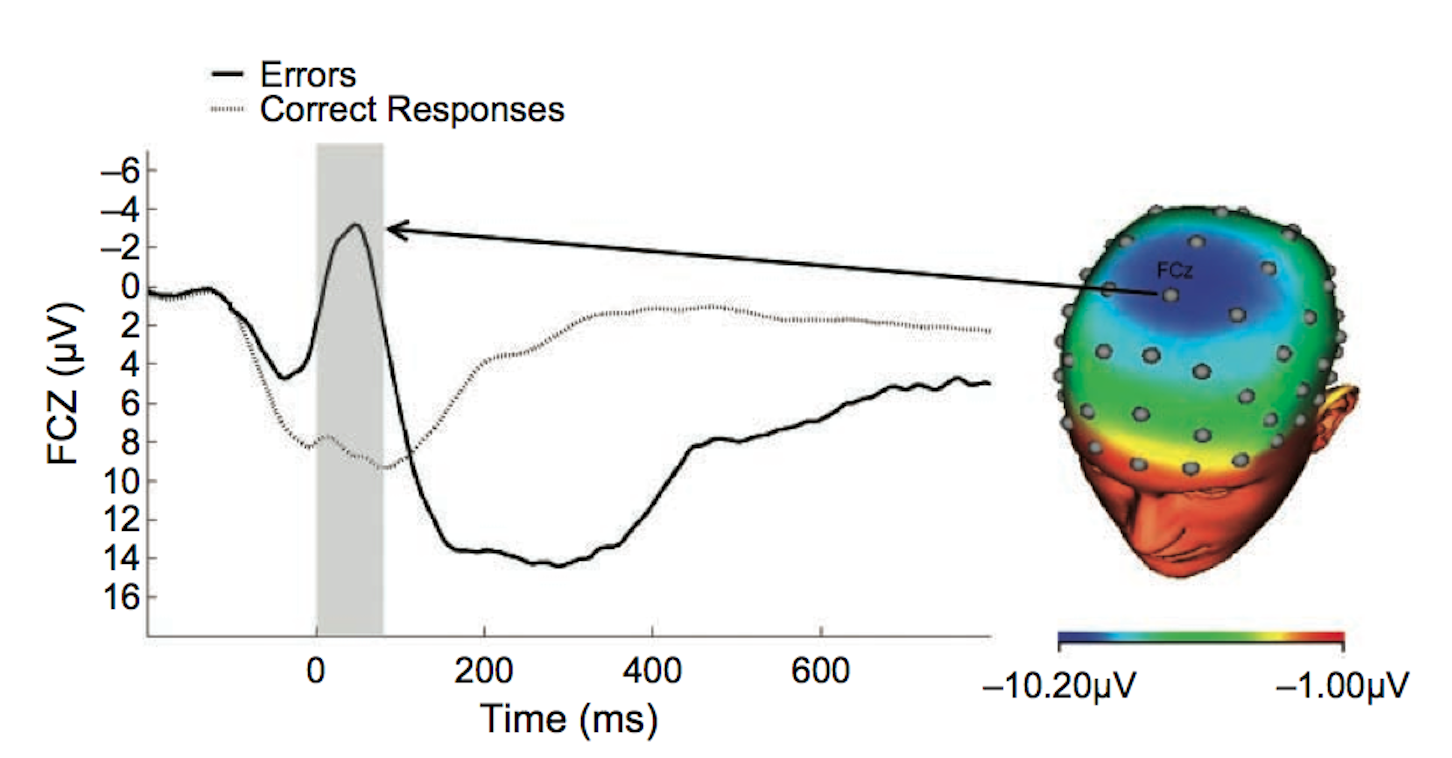
\includegraphics{ERN_voltage}
	     \caption{Mean event-related potentials time-locked to correct and erroneous responses at electrode FCz (left). This graph plots voltage over time, where the response occurs at 0 milliseconds (ms). The error-related negativity (ERN) is observed as a sharp negative deflection that peaks around 50 ms (illustrated by the gray bar) after the commission of a mistake.The voltage difference between errors and correct responses in the time window of the ERN can be plotted over the scalp (right); the ERN is maximal at the frontal-central midline of the scalp. Caption also from Figure 1 of Hajcak, 2012}
	 \label{ERN}
	\end{figure}

		\subsection{State versus Trait Anxiety}
		
A consensus as to the definition of emotions in general is still absent in the literature, but in the context of ERPs and their measures it makes sense to adopt a view seating emotion in motivational states and to define as parameters thereof direction -- away from or toward a stimulus -- and magnitude of motivation, commonly referred to as valence and arousal respectively \citep{ch16_oxford_2011}.

Most generally, state anxiety is differentiated from trait anxiety in its duration and relationship to stimuli: state anxiety can be a reaction to a threatening stimulus, but trait anxiety can be sustained in the absence of a particular cause \citep{endler_state_2001}. One measure used to differentiate between these is 40-item questionnaire called the Spielberger State-Trait Anxiety Inventory (STAI). Though it is among the longest- and most widely-used studies differentiating between these types of anxiety, it remains unclear whether the questions identifying trait anxiety are measuring depression \citep{bieling_state_1998}. However, their comorbidity and shared mechanisms -- neurophysiological and even genetic -- make these generally difficult to isolate \citep{andrews_bright_2009}.

Anxiety is uniquely suitable for ERP studies because other states are likelier to decay over as many trials as are necessary to obtain a meaningful EEG signal. Additionally, because of the difficulty generally in relying on self-report of affective states -- ERPs can serve as a useful complement in discerning causal relationships between stimuli and response \citep{ch16_oxford_2011}.

Evidence exists for a significant role of state anxiety in increasing vigilance in cognitive tasks, in that activity increases in the same region of the brain (i.e. the right ventrolateral prefrontal cortex (VLPFC)) during both exposure to threatening stimuli and during difficult vigilance tasks, e.g. when search stimuli are relatively difficult to distinguish from background stimuli, or when search criteria must be held in working memory for a long period of time \citep{aron_inhibition_2004}. The analytical rumination (AR) hypothesis posits this conditionally adaptive relationship and, on a longer time scale, an adaptive role for the frequently comorbid trait anxiety and depression in attentional control and sustained analysis of complex issues \citep{andrews_bright_2009}.
	\section{Open Science}
		\subsection{Historical Precedence}

Most published research findings, whether in medical or psychological science, are not replicable \citep{ioannidis_why_2005}. Many causes appear to contribute to the prevalence of nonreplication, and while analyses of extant publications are important in both understanding the kind and extent of such problems, an important complement to these endeavors is systematic replication.

\begin{table}[htdp] % begins the table floating environment. This enables LaTeX to fit the table where it works best and lets you add a caption.
\caption[Table 1]{Summary of reasons for retraction of 742 paper, 2000 - 10} 
% The words in square brackets of the caption command end up in the Table of Tables. The words in curly braces are the caption directly over the table.
\begin{center} 
% makes the table centered
\begin{tabular}{l l l} 
% the tabular environment is used to make the table itself. The {c c c c} specify that the table will have four columns and they will all be center-aligned. You can make the cell contents left aligned by replacing the Cs with Ls or right aligned by using Rs instead. Add more letters for more columns, and pipes (the vertical line above the backslash) for vertical lines. Another useful type of column is the p{width} column, which forces text to wrap within whatever width you specify e.g. p{1in}. Text will wrap badly in narrow columns though, so beware.
\toprule % a horizontal line, slightly thicker than \hline, depends on the booktabs package
  Reason for retraction & Retracted paper, n(\%) & IF, mean (SD) \\ % the first row of the table. Separate columns with ampersands and end the line with two backslashes. An environment begun in one cell will not carry over to adjacent rows.
  \midrule % another horizontal line
\bf{Fraud} & & \\ % another row
Fabrication & 111 (15.0) & 9.70 (11.49) \\
Falsification & 98 (13.2) & 8.01 (8.33)\\
\bf{Error} & & \\
Scientific mistake & 234 (31.5) & 10.60 (10.66) \\
Duplicate publication & 117 (15.8) & 3.18 (2.63) \\
Plagiarism & 107 (14.4) & 2.31 (1.90) \\
Ethical violations & 76 (10.2) & 5.74 (8.51) \\
Unstated reasons & 61 (8.2) & 5.08 (8.82) \\
Journal error & 27 (3.6) & 2.66 (2.21) \\
\bottomrule % yet another horizontal line
IF, impact factor
\end{tabular}
\end{center}
\label{inheritance} % labels are useful when you have more than one table or figure in your document. See our online documentation for more on this.
\end{table}


Among these causes are demands for increasingly small effect sizes \citep{taubes_epidemiology_1995}. Additionally, false positives abound in the literature because of the margin allowed by the ubiquitous \textless.05 \emph{p}-value criterion for publication \citep{ioannidis_why_2005}.

Outside of these previous issues, the structure of professional science today emphasizes publications and funding for which labs are competitive on the basis of positive findings -- met analyses find that statistically significant results are three times more likely to be published than papers affirming null results \citep{jennings_publication_2011}. Because it is circular to explain this disparity being caused by experimenters' desires to submit significant findings, it is also important to consider the roles that reviewers and editors have in preferring those significant findings: not only are concurrent articles differentially prioritized according to whether they report positive results, but positive results are privileged if found first irrespective of the frequency of null findings thereof following, a phenomenon called latent bias. To the extent that we assume reviewers across impact factors of journals are equally discriminating, the greater frequency of retractions in higher-impact journals \citep{fang_retracted_2011} supports this.

Transparency would address methodological problems across kind and degree, from innocuous problems of standardizing experimental conditions and protocols to outright forgery, and thanks to the internet, researchers interested in implementing these practices are able to find and coordinate. Some endeavors are ostensibly more social, e.g. ResearchGate, of note because it is a place where researchers whose articles have been published in journals allowing it can post their research for free. Others are concerned more with methodology:  reaching consensus that science needs to be more open is the first and simplest obstacle to proliferating the practice -- adoption in the community and standardization within and among practices proves to be much more complex. The Open Science Collaboration was founded to address this.
		
		\subsection{Open Science Collaboration}
		
The Open Science Collaboration consists of two projects, the Open Science Framework (OSF) and the Reproducibility Project. The OSF is infrastructure for collaboration, including version control, a centralized place for sharing and finding experimental materials, documenting work, and standardizing workflow.
		
		\subsection{The Reproducibility Project}
		
At the time of this writing, more than 70 scientists have joined a single endeavor to replicate experiments published in three prominent psychological science journals: \emph{Psychological Science}, the \emph{Journal of Personality and Social Psychology}, and the \emph{Journal of Experimental Psychology: Learning, Memory, and Cognition}. The purpose is not just to test reproducibility of published research findings, but to develop a methodology to improve it \citep{osc_open_2012}.

Most studies come from the fields of social and cognitive psychology because they do not require specialized equipment and are less expensive, and most replications are being conducted by undergraduate students \citep{carpenter_psychology_2012}. Though such a homogeneous research population presents its own problems, a significant advantage exists in limiting costs of such studies because it serves dual purposes, including training.


	
\chapter{The Replication}
    	\section{Methods}
		\subsection{The Task}
Participants performed a flanker task in which they viewed five horizontally aligned arrows on a computer screen. On each trial, participants were to specify the direction of the central arrow with the click of a left or right mouse button. Whether the central arrow was aligned with flankers was pseudorandomly chosen and of equal frequency. Trials on which central and flanker arrows were aligned will hereafter be called compatible, while trials on which the central and flanker arrows were not aligned will hereafter be called incompatible.

Each participant first performed one practice block of 30 trials followed by eight additional blocks of 30 trials. Stimuli (i.e. the arrows) were presented for 200 ms with an intertrial interval (ITI) that varied pseudorandomly from 500 to 1000 ms. At the end of each of these blocks, participants saw on the screen one of three messages according to performance: if 75\% accurate or below, they saw ``Please try to be more accurate"; if above 90\% they saw ``Please try to respond faster"; if between these levels of accuracy, they saw ``You're doing a great job."
		\subsection{Errors and EEG}
While performing this task each participant was monitored for his or her electroencephalographic (EEG) and electromyographic (EMG) activity using the EasyCap electrode cap and BrainAmps Standard system (Brain Products, Gilding, Germany). Recordings were taken from 96 scalp electrodes at equidistant positions as well as from two reference electrodes placed on the left and right mastoids. Electrooculogram (EOG) from blinks and other eye movements were recorded from four facial electrodes placed approximately 1 cm: above the right eye, below the right eye, left of the left eye, and right of the right eye. All bioelectric signals were digitized on a laboratory microcomputer using Recorder software (Brain Products). Sampling was at 1000 Hz.

Offline analysis was performed using Brain Vision Analyzer software (Brain Products, Gilching, Germany). Data was referenced to the numeric mean of the mastoids and band-pass filtered with cutoffs of 0.1 and 30 Hz. EEG was segmented for each trial, beginning 200 ms before response and continuing for 800 ms. It was corrected for blinks and eye movements using EMCP \citep{gratton_new_1983}.  The ERN was defined as the average activity in a 0- to 100-ms window following response onset on error trials, but it generally peaks approximately 50 ms following commission of an error. The ERN will also be statistically evaluated using either STATA or R, with Greenhouse-Geisser correction applied to p values associated with multiple degrees of freedom, repeated measures comparisons.
		\subsection{Startle and EMG}
When presented, startle probes consisted of a 50-ms 105-dB burst of white noise with instantaneous onset 300ms after response. They were presented on 10\% of all trials in the practice block. In the eight blocks following practice, they were presented on 50\% of error trials, 50\% of correct trials following errors, and a random 4\% of other correct trials.

Startle response was measured with two electrodes placed approximately 12 mm apart under each participant�s left eye on the obicularis muscle. Startle response EMG data was band-pass filtered (28�512 Hz; 24 dB/ octave roll-off), rectified, then low-pass filtered at 30 Hz (24 dB/ octave) and baseline-corrected. Response magnitude and latencies were quantified according to a peak in the 20- to 120-ms window after the startle probe was presented. It will be statistically evaluated using STATA or R, with Greenhouse-Geisser correction applied to p values associated with multiple degrees of freedom, repeated measures comparisons.
	\section{Results}
(Expected)

I expect to see a greater startle response following error trials and correct-following-error (also called "predictable" \citep{hajcak_errors_2008} trials. I also expect, past a certain threshold of ERN amplitude \citep{hajcak_what_2012}, a negative correlation between startle magnitude and ERN amplitude (negative because the ERN is itself negative). I will also examine whether magnitude of startle response corresponded to total number of errors.

	\section{Discussion}

\chapter{The Extension}
    	\section{Methods}

Following the replication, participants will be asked to complete the state-trait anxiety inventory (STAI), discussed at greater length in ``State versus Trait Anxiety." In this part of the experiment, the same eight blocks of 30 trials will be run again with exactly the same visual and auditory stimuli and probabilities thereof, but participants will earn or lose points based on the speed and accuracy of their responses. They will be notified of points lost or gained after each trial.

To manipulate performance anxiety, the point system will be changed halfway through the extension (order counterbalanced across subjects). In both conditions, subjects will start out with +20 points. In the low anxiety condition, subjects will receive +2 points for correct responses that are faster than their average RT (calculated during the replication section), +1 points for correct responses slower than their average RT, and -1 points for incorrect responses. In the high anxiety condition, +1 point will be awarded for correct/fast trials, -1 point for correct/slow trials, and -2 points for incorrect trials. Hence, by manipulating the chances of winning/losing points, we seek to decrease/increase state anxiety. Subjects will be informed at the outset that their points will be compared to other subjects in this same study and when the study is complete the highest scorer will win \$75 and the second highest scorer will win \$25.
	
	\section{Results}
(expected)

I expect to see in the extension a positive correlation between ERN amplitude and trait anxiety\citep{hajcak_what_2012} and, irrespective of that relationship, a positive correlation between startle magnitude and both state and trait anxiety \citep{grillon_fear_1993}. Additionally, I expect to see correlations between trait anxiety and degree of state anxiety induced by the extension.
	\section{Discussion}
	
\chapter{General Discussion}

\chapter{The Future of Open Science}
\citep{van_horn_why_2012}
%\chapter{Tables and Graphics}

%	\clearpage 
%% \clearpage ends the page, and also dumps out all floats. 
%% Floats are things like tables and figures.

%If you want to make a table that is longer than a page, you will want to use the longtable environment. Uncomment the table below to see an example, or see our online documentation.

%	\begin{longtable}{||c|c|c|c||}
%	 	\caption[Long Table]{An example of a long table, with headers that repeat on each subsequent page: Results from the summers of 1998 and 1999 work at Reed College done
%by Grace Brannigan, Robert Holiday and Lien Ngo in 1998 and Kate Brown and
%Christina Inman in 1999.}\\ \hline
%	    	  \multicolumn{4}{||c||}{Chromium Hexacarbonyl} \\\hline
%		   State & Laser wavelength & Buffer gas & Ratio of $\frac{\textrm{Intensity
%at vapor pressure}}{\textrm{Intensity at 240 Torr}}$ \\ \hline
%		  \endfirsthead
%		\hline     State & Laser wavelength & Buffer gas & Ratio of
%$\frac{\textrm{Intensity at vapor pressure}}{\textrm{Intensity at 240 Torr}}$\\
%\hline
%		    \endhead

%	    $z^{7}P^{\circ}_{4}$ & 266 nm & Argon & 1.5 \\\hline
%	    $z^{7}P^{\circ}_{2}$ & 355 nm & Argon & 0.57 \\\hline
%	    $y^{7}P^{\circ}_{3}$ & 266 nm & Argon & 1 \\\hline
%	    $y^{7}P^{\circ}_{3}$ & 355 nm & Argon & 0.14 \\\hline
%	    $y^{7}P^{\circ}_{2}$ & 355 nm & Argon & 0.14 \\\hline
%	    $z^{5}P^{\circ}_{3}$ & 266 nm & Argon & 1.2 \\\hline
%	    $z^{5}P^{\circ}_{3}$ & 355 nm & Argon & 0.04 \\\hline
%	    $z^{5}P^{\circ}_{3}$ & 355 nm & Helium & 0.02 \\\hline
%	    $z^{5}P^{\circ}_{2}$ & 355 nm & Argon & 0.07 \\\hline
%	    $z^{5}P^{\circ}_{1}$ & 355 nm & Argon & 0.05 \\\hline
%	    $y^{5}P^{\circ}_{3}$ & 355 nm & Argon & 0.05, 0.4 \\\hline
%	    $y^{5}P^{\circ}_{3}$ & 355 nm & Helium & 0.25 \\\hline
%	    $z^{5}F^{\circ}_{4}$ & 266 nm & Argon & 1.4 \\\hline
%	    $z^{5}F^{\circ}_{4}$ & 355 nm & Argon & 0.29 \\\hline
%	    $z^{5}F^{\circ}_{4}$ & 355 nm & Helium & 1.02 \\\hline
%	    $z^{5}D^{\circ}_{4}$ & 355 nm & Argon & 0.3 \\\hline
%	    $z^{5}D^{\circ}_{4}$ & 355 nm & Helium & 0.65 \\\hline
%	    $y^{5}H^{\circ}_{7}$ & 266 nm & Argon & 0.17 \\\hline
%	    $y^{5}H^{\circ}_{7}$ & 355 nm & Argon & 0.13 \\\hline
%	    $y^{5}H^{\circ}_{7}$ & 355 nm & Helium & 0.11 \\\hline
%	    $a^{5}D_{3}$ & 266 nm & Argon & 0.71 \\\hline
%	    $a^{5}D_{2}$ & 266 nm & Argon & 0.77 \\\hline
%	    $a^{5}D_{2}$ & 355 nm & Argon & 0.63 \\\hline
%	    $a^{3}D_{3}$ & 355 nm & Argon & 0.05 \\\hline
%	    $a^{5}S_{2}$ & 266 nm & Argon & 2 \\\hline
%	    $a^{5}S_{2}$ & 355 nm & Argon & 1.5 \\\hline
%	    $a^{5}G_{6}$ & 355 nm & Argon & 0.91 \\\hline
%	    $a^{3}G_{4}$ & 355 nm & Argon & 0.08 \\\hline
%	    $e^{7}D_{5}$ & 355 nm & Helium & 3.5 \\\hline
%	    $e^{7}D_{3}$ & 355 nm & Helium & 3 \\\hline
%	    $f^{7}D_{5}$ & 355 nm & Helium & 0.25 \\\hline
%	    $f^{7}D_{5}$ & 355 nm & Argon & 0.25 \\\hline
%	    $f^{7}D_{4}$ & 355 nm & Argon & 0.2 \\\hline
%	    $f^{7}D_{4}$ & 355 nm & Helium & 0.3 \\\hline
%	    \multicolumn{4}{||c||}{Propyl-ACT} \\\hline
%	    State & Laser wavelength & Buffer gas & Ratio of $\frac{\textrm{Intensity
%at vapor pressure}}{\textrm{Intensity at 240 Torr}}$\\ \hline
%	    $z^{7}P^{\circ}_{4}$ & 355 nm & Argon & 1.5 \\\hline
%	    $z^{7}P^{\circ}_{3}$ & 355 nm & Argon & 1.5 \\\hline
%	    $z^{7}P^{\circ}_{2}$ & 355 nm & Argon & 1.25 \\\hline
%	    $z^{7}F^{\circ}_{5}$ & 355 nm & Argon & 2.85 \\\hline
%	    $y^{7}P^{\circ}_{4}$ & 355 nm & Argon & 0.07 \\\hline
%	    $y^{7}P^{\circ}_{3}$ & 355 nm & Argon & 0.06 \\\hline
%	    $z^{5}P^{\circ}_{3}$ & 355 nm & Argon & 0.12 \\\hline
%	    $z^{5}P^{\circ}_{2}$ & 355 nm & Argon & 0.13 \\\hline
%	    $z^{5}P^{\circ}_{1}$ & 355 nm & Argon & 0.14 \\\hline
%	    \multicolumn{4}{||c||}{Methyl-ACT} \\\hline
%	    State & Laser wavelength & Buffer gas & Ratio of $\frac{\textrm{Intensity
%at vapor pressure}}{\textrm{Intensity at 240 Torr}}$\\ \hline
%	    $z^{7}P^{\circ}_{4}$ & 355 nm & Argon & 1.6, 2.5 \\\hline
%	    $z^{7}P^{\circ}_{4}$ & 355 nm & Helium & 3 \\\hline
%	    $z^{7}P^{\circ}_{4}$ & 266 nm & Argon & 1.33 \\\hline
%	    $z^{7}P^{\circ}_{3}$ & 355 nm & Argon & 1.5 \\\hline
%	    $z^{7}P^{\circ}_{2}$ & 355 nm & Argon & 1.25, 1.3 \\\hline
%	    $z^{7}F^{\circ}_{5}$ & 355 nm & Argon & 3 \\\hline
%	    $y^{7}P^{\circ}_{4}$ & 355 nm & Argon & 0.07, 0.08 \\\hline
%	    $y^{7}P^{\circ}_{4}$ & 355 nm & Helium & 0.2 \\\hline
%	    $y^{7}P^{\circ}_{3}$ & 266 nm & Argon & 1.22 \\\hline
%	    $y^{7}P^{\circ}_{3}$ & 355 nm & Argon & 0.08 \\\hline
%	    $y^{7}P^{\circ}_{2}$ & 355 nm & Argon & 0.1 \\\hline
%	    $z^{5}P^{\circ}_{3}$ & 266 nm & Argon & 0.67 \\\hline
%	    $z^{5}P^{\circ}_{3}$ & 355 nm & Argon & 0.08, 0.17 \\\hline
%	    $z^{5}P^{\circ}_{3}$ & 355 nm & Helium & 0.12 \\\hline
%	    $z^{5}P^{\circ}_{2}$ & 355 nm & Argon & 0.13 \\\hline
%	    $z^{5}P^{\circ}_{1}$ & 355 nm & Argon & 0.09 \\\hline
%	    $y^{5}H^{\circ}_{7}$ & 355 nm & Argon & 0.06, 0.05 \\\hline
%	    $a^{5}D_{3}$ & 266 nm & Argon & 2.5 \\\hline
%	    $a^{5}D_{2}$ & 266 nm & Argon & 1.9 \\\hline
%	    $a^{5}D_{2}$ & 355 nm & Argon & 1.17 \\\hline
%	    $a^{5}S_{2}$ & 266 nm & Argon & 2.3 \\\hline
%	    $a^{5}S_{2}$ & 355 nm & Argon & 1.11 \\\hline
%	    $a^{5}G_{6}$ & 355 nm & Argon & 1.6 \\\hline
%	    $e^{7}D_{5}$ & 355 nm & Argon & 1 \\\hline

%		\end{longtable}

   
 %%  \section{Figures}
   
%	If your thesis has a lot of figures, \LaTeX\ might behave better for you than that other word processor.  One thing that may be annoying is the way it handles ``floats'' like tables and figures. \LaTeX\ will try to find the best place to put your object based on the text around it and until you're really, truly done writing you should just leave it where it lies.   There are some optional arguments to the figure and table environments to specify where you want it to appear; see the comments in the first figure.

%	If you need a graphic or tabular material to be part of the text, you can just put it inline. If you need it to appear in the list of figures or tables, it should be placed in the floating environment. 
	
%	To get a figure from StatView, JMP, SPSS or other statistics program into a figure, you can print to pdf or save the image as a jpg or png. Precisely how you will do this depends on the program: you may need to copy-paste figures into Photoshop or other graphic program, then save in the appropriate format.
	
%	Below we have put a few examples of figures. For more help using graphics and the float environment, see our online documentation.
	
%	And this is how you add a figure with a graphic:
%	\begin{figure}[h]
	% the options are h = here, t = top, b = bottom, p = page of figures.
	% you can add an exclamation mark to make it try harder, and multiple
	% options if you have an order of preference, e.g.
	% \begin{figure}[h!tbp]
	   
%	       \centering
	    % DO NOT ADD A FILENAME EXTENSION TO THE GRAPHIC FILE
%	    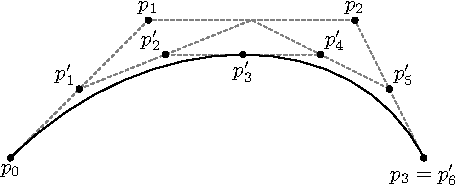
\includegraphics{subdivision}
%	     \caption{A Figure}
%	 \label{subd}
%	\end{figure}

%\clearpage %% starts a new page and stops trying to place floats such as tables and figures

%\section{More Figure Stuff}
%You can also scale and rotate figures.
% 	\begin{figure}[h!]
	   
%	       \centering
	    % DO NOT ADD A FILENAME EXTENSION TO THE GRAPHIC FILE
%	    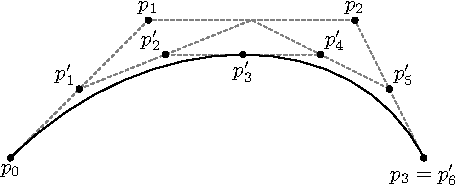
\includegraphics[scale=0.5,angle=180]{subdivision}
	    % if your figure shows up not where you want it, it may just be too big to fit. You can use the scale argument to shrink it, e.g. scale=0.85 is 85 percent of the original size. 
%	     \caption{A Smaller Figure, Flipped Upside Down}
%	 \label{subd2}
%	\end{figure}

%\section{Even More Figure Stuff}
%With some clever work you can crop a figure, which is handy if (for instance) your EPS or PDF is a little graphic on a whole sheet of paper. The viewport arguments are the lower-left and upper-right coordinates for the area you want to crop.

% 	\begin{figure}[h!]
%	    	       \centering
%	    % DO NOT ADD A FILENAME EXTENSION TO THE GRAPHIC FILE
%	   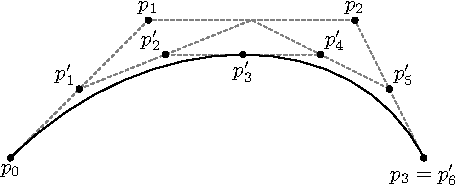
\includegraphics[clip=true, viewport=.0in .0in 1in 1in]{subdivision}
%	    \caption{A Cropped Figure}
%	 \label{subd3}
%	\end{figure}
%	
%      \subsection{Common Modifications}
%      The following figure features the more popular changes thesis students want to their figures. This information is also on the web at \url{web.reed.edu/cis/help/latex/graphics.html}.
%           \renewcommand{\thefigure}{0.\arabic{figure}} %Renumbers the figure to the type 0.x
%    \addtocounter{figure}{4} %starts the figure numbering at 4
%    \begin{figure}[htbp]
%    \begin{center}
%   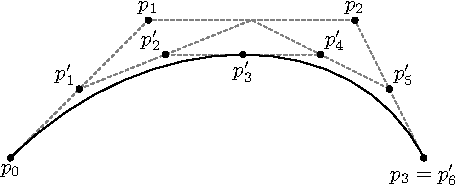
\includegraphics[scale=0.5]{subdivision}
%    \caption[Flower type and percent specialization]{\footnotesize{Interaction bar plot showing the degree of specialization for each flower type.}} %the special ToC caption is in square brackets. The \footnotesize makes the figure caption smaller
%    \label{barplot}
%    \end{center}
%    \end{figure} 

\chapter*{Conclusion}
         \addcontentsline{toc}{chapter}{Conclusion}
	\chaptermark{Conclusion}
	\markboth{Conclusion}{Conclusion}
	\setcounter{chapter}{4}
	\setcounter{section}{0}
	
Here's a conclusion, demonstrating the use of all that manual incrementing and table of contents adding that has to happen if you use the starred form of the chapter command. The deal is, the chapter command in \LaTeX\ does a lot of things: it increments the chapter counter, it resets the section counter to zero, it puts the name of the chapter into the table of contents and the running headers, and probably some other stuff. 

So, if you remove all that stuff because you don't like it to say ``Chapter 4: Conclusion'', then you have to manually add all the things \LaTeX\ would normally do for you. Maybe someday we'll write a new chapter macro that doesn't add ``Chapter X'' to the beginning of every chapter title.

\section{More info}
And here's some other random info: the first paragraph after a chapter title or section head \emph{shouldn't be} indented, because indents are to tell the reader that you're starting a new paragraph. Since that's obvious after a chapter or section title, proper typesetting doesn't add an indent there. 


%If you feel it necessary to include an appendix, it goes here.
    \appendix
      \chapter{The First Appendix}
      \chapter{The Second Appendix, for Fun}


%This is where endnotes are supposed to go, if you have them.
%I have no idea how endnotes work with LaTeX.

  \backmatter % backmatter makes the index and bibliography appear properly in the t.o.c...



% if you're using bibtex, the next line forces every entry in the bibtex file to be included
% in your bibliography, regardless of whether or not you've cited it in the thesis.
\bibliography{thesis}                                                                                                                                                \bibliographystyle{APA/apa-good}                                                                                                                                                                              %\nocite{*}
% Finally, an index would go here... but it is also optional.
\end{document}
